\documentclass{IEEEtaes}

% Packages kept to the template set plus standard math/figure packages that
% are available in every TeX Live distribution used by Overleaf.
\usepackage{color,array,amsthm}
\usepackage{graphicx}
\usepackage{amsmath,amssymb}
\usepackage[dvipsnames]{xcolor}
\usepackage{algorithm}
\usepackage{algpseudocode}

\jvol{XX}
\jnum{XX}
\jmonth{XXXXX}
\paper{1234567}
\pubyear{2026}
\doiinfo{TAES.2026.Doi Number}

\newtheorem{assumption}{Assumption}
\newtheorem{definition}{Definition}
\newtheorem{lemma}{Lemma}
\newtheorem{proposition}{Proposition}
\newtheorem{property}{Property}
\newtheorem{remark}{Remark}
\setcounter{page}{1}
% Cross-references to subsections read ``Section~III-C''.
\makeatletter
\renewcommand{\p@subsection}{\thesection-}
\makeatother

% ---------------------------------------------------------------------------
% Notation and helper macros (single source for symbols used in the paper)
% ---------------------------------------------------------------------------

% Placeholder for content that waits for the formal results or author input.
\newcommand{\todo}[1]{{\color{red}[\textbf{TODO:} #1]}}

% Generic
\newcommand{\R}{\mathbb{R}}
\newcommand{\SE}{\mathrm{SE}(3)}
\newcommand{\SO}{\mathrm{SO}(3)}
\newcommand{\T}{\top}
\newcommand{\E}{\mathbb{E}}
\newcommand{\norm}[1]{\left\lVert #1 \right\rVert}
\newcommand{\clip}{\operatorname{clip}}
\newcommand{\diag}{\operatorname{diag}}
\newcommand{\argmin}{\operatorname*{arg\,min}}
\newcommand{\lexmin}{\operatorname*{lex\,min}}

% Frames
\newcommand{\FI}{\mathcal{F}_{I}}
\newcommand{\FT}{\mathcal{F}_{T}}
\newcommand{\FC}{\mathcal{F}_{C}}
\newcommand{\FL}{\mathcal{F}_{L}}

% Mission
\newcommand{\Td}{T_{d}}            % mission deadline
\newcommand{\Dd}{\Delta_{d}}       % terminal reserve
\newcommand{\Lt}{L}                % latest admissible entry time
\newcommand{\Bmax}{B_{\max}}       % Delta-v budget
\newcommand{\dvused}{\Delta v_{\mathrm{u}}} % Delta-v used so far

% Geometry
\newcommand{\shat}{\hat{s}}
\newcommand{\er}{e_{r}}
\newcommand{\epol}{e_{\mathrm{pol}}}
\newcommand{\eaz}{e_{\mathrm{az}}}
\newcommand{\dlat}{\Delta\lambda}
\newcommand{\thg}{\theta_{g}}
\newcommand{\Tset}{\mathcal{T}}          % entry arrival-time candidates
\newcommand{\Wgeo}{\mathcal{W}_{\mathrm{geo}}}
\newcommand{\vb}{v_{b}}                  % braking envelope

% Decision and execution
\newcommand{\Bgrid}{\mathfrak{B}}        % candidate intent grid
\newcommand{\Bc}{\mathfrak{B}_{c}}       % certifiable candidate set
\newcommand{\Cmap}{\mathcal{C}}          % certification map
\newcommand{\zE}{z_{E}}                  % execution feedback
\newcommand{\PE}{P_{\mathcal{E}}}        % execution-layer macro kernel
\newcommand{\PC}{P_{\mathcal{C}}}        % certification-induced kernel
\newcommand{\gd}{\gamma_{d}}             % per-decision discount
\newcommand{\Hp}{H_{p}}                  % mode-prediction horizon
\newcommand{\ehat}{\hat{e}}
\newcommand{\tauhat}{\hat{\tau}}
\newcommand{\dvhat}{\widehat{\Delta v}}
\newcommand{\rtil}{\tilde{r}}

% Method names (fixed terminology, see fact sheet 00)
\newcommand{\ECC}{ECC}
\newcommand{\RWG}{RWG}


\raggedbottom
% Float placement: allow several floats per page in the results section.
\renewcommand{\topfraction}{0.9}\renewcommand{\bottomfraction}{0.6}\renewcommand{\textfraction}{0.08}
\renewcommand{\floatpagefraction}{0.8}\renewcommand{\dbltopfraction}{0.9}\renewcommand{\dblfloatpagefraction}{0.8}
\setcounter{topnumber}{3}\setcounter{bottomnumber}{2}\setcounter{totalnumber}{5}\setcounter{dbltopnumber}{2}
\begin{document}

\title{Execution-Feedback Closed-Loop Coordination of Reinforcement Learning and Model Predictive Control for Pre-Capture Approach to a Fast-Tumbling Target}

\author{\todo{AUTHOR NAMES}}
\affil{Hohai University, Changzhou, China}

\receiveddate{Manuscript received XXXXX 00, 0000; revised XXXXX 00, 0000; accepted XXXXX 00, 0000.\\
\todo{Funding information.}}

\corresp{\todo{Corresponding author.}}

\authoraddress{\todo{Author affiliations and e-mail addresses.}}

\markboth{AUTHOR ET AL.}{EXECUTION-FEEDBACK RL--MPC COORDINATION FOR TUMBLING-TARGET PRE-CAPTURE}
\maketitle

\begin{abstract}
\todo{Abstract: written after the formal results are delivered. Planned content: decision--execution mismatch in learning-guided MPC for fast-tumbling-target pre-capture; ECC (execution-opportunity coordination of the proposed intent and learning on the coordinated closed loop) and RWG; six-degree-of-freedom simulation of time-limited capture; key results.}
\end{abstract}

\begin{IEEEkeywords}
\todo{Keywords, alphabetical: e.g., model predictive control, non-cooperative target, reinforcement learning, rendezvous and proximity operations, tumbling target.}
\end{IEEEkeywords}

\section{INTRODUCTION}\label{sec:intro}

\IEEEPARstart{O}{n-orbit} servicing and the removal of failed spacecraft require a servicing spacecraft to approach a target autonomously and to establish the relative position, attitude, and velocity needed for capture \cite{tian2024taes}. In this pre-capture phase, the chaser must respect a safe distance, a narrow approach corridor, the field of view of its camera, relative-speed limits, and its actuator capability, so that a capture window opens \cite{lian2026asr}. A noncooperative target, such as a failed spacecraft \cite{xu2026ast}, offers no assistance: its docking interface moves with the tumbling body, and the chaser must coordinate its relative position and attitude with a moving capture point rather than a fixed one \cite{dong2025aa,wang2026ast}. Fast tumbling turns this into a timing problem. When the target tumbles at $2$--$3^{\circ}$/s, the port faces the chaser only once per spin period of about two and a half minutes; with a deadline and a propellant budget, this period is comparable to the deadline. The feasible capture window then varies with time and is scarce: a missed pass costs a full spin period, and whether the next pass is usable depends on the approach speed and timing chosen tens of seconds before it.

Constrained approaches to tumbling targets are commonly solved by model predictive control (MPC) or trajectory optimization. A two-stage MPC brings the chaser into a time-varying line-of-sight region and then tracks the periodic motion of the port \cite{dong2022aa}; tube MPC with online inertia estimation accounts for the limited predictability of the tumbling \cite{dong2024asr}; a dual-layer MPC filters nominal commands with control barrier functions \cite{xu2026ast}; second-order cone MPC encodes corridor and pointing requirements as convex constraints \cite{lian2026asr}; and manifold-based planning computes soft-docking trajectories \cite{wang2026ast}. These methods enforce the constraints explicitly over their prediction horizons and reach the port by converging to its periodic motion or by tracking it within one alignment. They consider moderate tumbling rates, such as about $1^{\circ}$/s \cite{tian2024taes}, or tasks without a deadline and budget \cite{dong2024asr}, in which a missed alignment can be awaited, and their long-horizon performance relies on the reference and terminal design \cite{xu2026ast}. Which pass to use, and how to arrive at it in time, lies beyond the horizon of such an optimization.

Reinforcement learning (RL), in contrast, learns state-dependent policies from interaction with the objective of the whole task. Deep RL algorithms such as soft actor--critic (SAC) \cite{haarnoja2018sac} and TD3 \cite{fujimoto2018td3} have controlled six-degree-of-freedom rendezvous with a rotating target end to end \cite{yang2025taes}, and hierarchical and safe RL have been applied to small-satellite guidance and to attitude tracking of noncooperative targets \cite{tammam2025cep,lu2026ast}; under complex constraints, however, exploration efficiency and execution reliability remain limited. MPC and RL thus have nearly complementary properties \cite{reiter2026arc,reiter2025ac4mpc}, and their combinations can be grouped by what the learned component provides to the optimizer \cite{reiter2026arc}. Learning can supply value and cost information: the terminal value, the cost, or the initial guess of an MPC \cite{reiter2025ac4mpc,ghezzi2026ecc,gong2026ast}, value targets from model predictions \cite{wu2024mpcvalue}, or MPC-shaped rewards for docking \cite{ramezani2026aa}. Learning can also supply task references and timing to an MPC that performs the constrained execution, such as maneuver times \cite{ren2026taes} and re-optimization instants \cite{zheng2026aa}, or coordinate the authority of learned and model-based controllers by flight phase \cite{adjei2026ast}. This article belongs to the second group: the learned layer sets stage targets, and the executor is part of its environment \cite{reiter2026arc}. In such schemes a learned decision is executed as issued, and its consequence reaches learning only through the return; where the executor may change a decision, it does so for safety or feasibility, as in shields \cite{alshiekh2018shielding}, feasibility and reference governors \cite{leung2024scl,tartaglione2024aut,duan2025autcon}, and safe-evolving or residual RL \cite{lu2025eaai,zeng2026neucom}.

Fast-tumbling pre-capture under a deadline leaves two problems open in these architectures. The first is the use of the dynamic capture window. Whether a pass is usable depends on how closely the line of sight approaches the cone swept by the port, and when it occurs depends on the phase of the port; a locally feasible approach does not imply that a pass is reached before the deadline. The decisions of the learned layer must therefore act on these quantities. The second is the coordination between long-horizon decisions and short-horizon constrained execution. Whether a decision is converted into an entry is resolved by the planning, gating, and tracking of the executor within seconds, whereas the decision layer acts once per stage and the outcome, capture or timeout, appears much later. When passes are scarce, neighboring decisions lead to capture and to timeout, so that the value of a decision changes abruptly across the action space at boundaries set by the executor. Such a value is hard to learn from the sparse terminal return, and a modification aimed at safety or feasibility leaves a safe decision unchanged even when it misses the last usable opportunity.

This article addresses the two problems with a hierarchical framework in which a learned policy issues two-dimensional stage intents to an execution layer of planners and MPC. Rotation-synchronized window guidance (RWG) turns each intent into stage goals that regulate the line of sight onto the sweep cone of the port and set the closing pace and the timing of the encounter, and it plans and re-times entries toward the predicted port motion. Execution-feedback closed-loop coordination (ECC) lets the execution layer predict, at every decision, the entry opportunities that it can realize, selects the executed object from the proposal and these opportunities by a fixed rule, and trains the policy on the resulting closed loop. The main contributions are as follows.
\begin{enumerate}
\item An execution-opportunity coordination of learning and constrained execution. At every decision, the execution layer predicts with its own models whether the proposed intent and a grid of alternatives lead to an entry, and whether an entry can still be planned directly at the last usable pass; one rule keeps the proposal, corrects it at a critical window, or launches the direct entry. SAC is trained on the coordinated closed loop with the proposals stored, so that the critics evaluate what happens when the policy proposes an intent, with the losses of standard SAC. In contrast to shields and governors \cite{alshiekh2018shielding,leung2024scl,lu2025eaai}, the coordination acts on task opportunities rather than on safety or feasibility, and in contrast to model-based value estimation \cite{wu2024mpcvalue}, the execution layer generates no value targets.
\item A rotation-synchronized window guidance derived from the sweep-cone geometry of the port. It characterizes the passing window by the latitude offset and the phase of the line of sight, regulates the latitude by a fixed law, and leaves the closing pace and the along-sweep timing to the policy; entries are gated on the predicted arrival and re-timed within the same pass. Unlike multistage MPC that converges to the periodic motion of the port \cite{dong2022aa}, RWG schedules the encounter with a pass that may not recur before the deadline.
\item A validation in six-degree-of-freedom simulations of time-limited pre-capture with gravity gradient and $J_{2}$ perturbation, with safety judged on the true trajectory and the dynamic model of \cite{yang2025taes}. On paired test tasks, ECC captures $85.4\%$ of the tasks, $11.6$ percentage points more than learning-guided MPC on the same execution chain at comparable time and propellant cost, and it retains this capture rate under a slower spin and a stronger nutation outside the training distribution.
\end{enumerate}

The remainder of this article is organized as follows. Section~\ref{sec:problem} formulates the pre-capture problem. Section~\ref{sec:framework} presents the hierarchical framework and RWG. Section~\ref{sec:ecc} develops ECC. Section~\ref{sec:experiments} reports the numerical study, and Section~\ref{sec:conclusion} concludes the article.

\textit{Notations:} Bold lowercase and uppercase symbols denote vectors and matrices, $\norm{\cdot}$ is the Euclidean norm, $\norm{\vect{y}}_{\vect{W}}^{2}=\vect{y}^{\T}\vect{W}\vect{y}$, $\bI_{3}$ is the identity matrix, $\vect{1}$ is the vector of ones, $\vect{y}_{1}^{\times}$ is the skew-symmetric matrix with $\vect{y}_{1}^{\times}\vect{y}_{2}=\vect{y}_{1}\times\vect{y}_{2}$, $(\cdot)^{\wedge}$ maps a twist to $\mathfrak{se}(3)$, $\log$ is the matrix logarithm on $\SO$ and $(\cdot)^{\vee}$ the inverse of $(\cdot)^{\times}$, and $\angle(\vect{y}_{1},\vect{y}_{2})$ is the angle between two vectors. $\norm{\cdot}_{\infty}$ is the maximum norm, and the saturation $\sat(\vect{y};\bar y)=\vect{y}\min\{1,\bar y/\norm{\vect{y}}\}$ for $\vect{y}\neq\vect{0}$, with $\sat(\vect{0};\bar y)=\vect{0}$, applies to scalars and vectors. A hat denotes a predicted quantity, a bar an upper bound, and a tilde a transformed quantity; $\Delta$ denotes increments only.

\section{PROBLEM FORMULATION}\label{sec:problem}

The pre-capture phase starts with the chaser some ten meters away from a freely tumbling, noncooperative target and ends when the chaser holds a capture pose in front of the target docking port. This section states the dynamics and the prediction model available to the chaser, the capture geometry and the safety constraints, and the resulting optimization problem, and it closes with an analysis of the features that shape the methods of Sections~\ref{sec:framework} and~\ref{sec:ecc}.

\subsection{Dynamics and Prediction Model}\label{sec:dynamics}

Three right-handed frames are used (Fig.~\ref{fig:scene}): the Earth-centered inertial frame $\FI$, the target body frame $\FT$ aligned with the principal axes of the target, and the chaser body frame $\FC$, whose $x$-axis, with unit vector $\vect{e}_{\mathrm{C}}$, is the camera boresight. The configuration of each spacecraft is described on the Lie group $\SE$, which represents attitude and position jointly and without singularities \cite{yang2025taes,gong2026ast}. The pose is $\bg=(\bR,\bp)\in\SE$, where $\bR\in\SO$ maps the body frame to $\FI$ and $\bp\in\R^{3}$ is the inertial position, and the body twist is $\bxi=[\bw^{\T},\bnu^{\T}]^{\T}$ with angular velocity $\bw$ and translational velocity $\bnu$. Following \cite{yang2025taes}, the motion of each rigid body obeys
\begin{align}
\dot{\bg} &= \bg\,\bxi^{\wedge}, \label{eq:kin}\\
\bJ\dot{\bw} &= -\bw\times\bJ\bw+\bG_{\mathrm{g}}+\bG, \label{eq:rot}\\
m\dot{\bnu} &= -m\,\bw\times\bnu+\bff_{\mathrm{g}}+\bff, \label{eq:trans}
\end{align}
where $m$ and $\bJ$ are the mass and the inertia matrix and $(\bG,\bff)$ is the control wrench in the body frame. With $\bp_{\mathrm{b}}=\bR^{\T}\bp$, $p=\norm{\bp}$, and $\bM=\tfrac12\mathrm{tr}(\bJ)\bI_{3}-\bJ$, the gravitational wrench consists of the gravity-gradient torque and the central force with its second-order mass-moment correction and the $J_{2}$ perturbation \cite{yang2025taes,tian2024taes},
\begin{align}
\bG_{\mathrm{g}} &= \frac{3\mu}{p^{5}}\,\bp_{\mathrm{b}}\times\bJ\bp_{\mathrm{b}},\label{eq:tg}\\
\bff_{\mathrm{g}} &= -\frac{\mu m}{p^{3}}\bp_{\mathrm{b}}-\frac{3\mu}{p^{5}}\bM\bp_{\mathrm{b}}+\frac{15\mu\,\bp_{\mathrm{b}}^{\T}\bM\bp_{\mathrm{b}}}{2p^{7}}\bp_{\mathrm{b}}+\bR^{\T}\bff_{J_{2}},\label{eq:fg}
\end{align}
where $\mu$ is the gravitational parameter of the Earth and $\bff_{J_{2}}$ is the $J_{2}$ force in $\FI$. The subscripts $\mathrm{T}$ and $\mathrm{C}$ refer to the target and the chaser. The relative pose and twist are $\bg_{\mathrm{r}}=\bg_{\mathrm{T}}^{-1}\bg_{\mathrm{C}}$ and $\bxi_{\mathrm{r}}=\bxi_{\mathrm{C}}-\mathrm{Ad}_{\bg_{\mathrm{r}}^{-1}}\bxi_{\mathrm{T}}$; their exponential coordinates form the relative state used by the near-field controller. The relative position is $\brho=\bp_{\mathrm{C}}-\bp_{\mathrm{T}}$ with range $\rho=\norm{\brho}$ and velocity $\bv=\dot{\brho}$, and $\brhoT=\bR_{\mathrm{T}}^{\T}\brho$ is the same position expressed in $\FT$. The joint state of the two spacecraft is denoted by $X=(\bg_{\mathrm{T}},\bxi_{\mathrm{T}},\bg_{\mathrm{C}},\bxi_{\mathrm{C}})$.

The control wrench is held constant over each control period $\Delta t$ and is bounded per axis by $\norm{\bff}_{\infty}\le\fmax$ and $\norm{\bG}_{\infty}\le\Gmax$. The propellant used up to time $t$ is measured by the velocity increment
\begin{equation}\label{eq:dv}
\Delta v(t)=\int_{0}^{t}\frac{\norm{\bff_{\mathrm{C}}(t')}}{\mC}\,\dd t'.
\end{equation}

\begin{assumption}\label{ass:info}
The relative state and the attitude and angular velocity of the target are measured; the inertia of the target is unknown to the chaser.
\end{assumption}

Under Assumption~\ref{ass:info}, every prediction of the target attitude used for decision and planning holds the current angular velocity constant,
\begin{equation}\label{eq:pred}
\hat{\bR}_{\mathrm{T}}(t+\tau)=\bR_{\mathrm{T}}(t)\exp\bigl(\tau\,\bw_{\mathrm{T}}(t)^{\times}\bigr),\qquad \tau\ge0,
\end{equation}
which is the torque-free motion of a body with isotropic inertia. The prediction rotates the target about the inertial spin axis $\bs=\bR_{\mathrm{T}}\bw_{\mathrm{T}}/\Omega$ at the spin rate $\Omega=\norm{\bw_{\mathrm{T}}}$ with spin period $\Ts=2\pi/\Omega$. The translational model used for planning is the double integrator
\begin{equation}\label{eq:di}
\ddot{\brho}=\bff/\mC
\end{equation}
in inertial axes, which neglects the differential gravity over the short ranges considered. Only the dynamics \eqref{eq:kin}--\eqref{eq:fg} use the true inertia.

\begin{figure}[t]
\centering
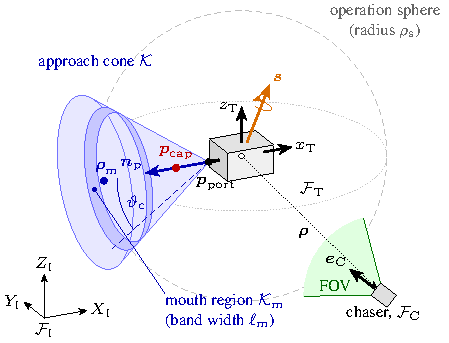
\includegraphics{figures/fig_scene.pdf}
\caption{Pre-capture scene (target enlarged for legibility). The port and the capture point are fixed in $\FT$ and rotate with the target about the spin axis $\bs$; the approach cone $\Kset$ of half-angle $\vartheta_{\mathrm{c}}$ opens along the port axis $\bnp$, and the operation sphere of radius $\rhos$ surrounds the target.}
\label{fig:scene}
\end{figure}

\subsection{Capture Geometry and Constraints}\label{sec:constraints}

The docking port $\bpport$, its approach axis $\bnp$, and the capture point $\bpcap$ are fixed in $\FT$, with $\bpport$ and $\bpcap$ on the port axis. The port direction in $\FI$ is $\bn=\bR_{\mathrm{T}}\bnp$; since the target tumbles, the capture point moves in $\FI$ and the chaser must meet a rotating interface rather than a fixed point. With the axial coordinate $\ell(\vect{u})=\bnp^{\T}(\vect{u}-\bpport)$, the approach cone is
\begin{equation}\label{eq:cone}
\begin{aligned}
\Kset=\bigl\{\vect{u}\in\R^{3}:\ &\ell(\vect{u})\ge\ell_{\min},\\
&\norm{\vect{u}-\bpport-\ell(\vect{u})\bnp}\le\ell(\vect{u})\tan\vartheta_{\mathrm{c}}\bigr\}.
\end{aligned}
\end{equation}
The operation sphere is the ball of radius $\rhos$ about the target center, and the mouth region $\Km=\{\brhoT\in\Kset:\rho<\rhos+\ell_{\mathrm{m}}\}$ extends it by a band of width $\ell_{\mathrm{m}}$ inside the cone. Approach speeds are limited by the braking envelope $\vb(\ell)$, a piecewise-linear inner approximation of the constant-deceleration profile $\sqrt{v_{\mathrm{f}}^{2}+\fmax\ell/\mC}$; every segment is a chord of this concave profile, so that $\vb$ is nowhere looser than it.

The safe set $\Sset$ is the set of joint states $X$ that satisfy the constraints of Table~\ref{tab:constraints}, where $d_{\mathrm{clr}}$ is the clearance between the envelope sphere of the chaser and the target body including its grapple rod, the radial closing speed $-\dot\rho$ is measured in $\FI$, and the speeds in $\Km$ are measured relative to the rotating target. The classification follows \cite{tian2024taes,xu2026ast}; actuator saturation is a limit, not a constraint violation. The capture set $\Xcap$ contains the joint states with $\brhoT\in\Kset$ whose position, attitude, velocity, and angular-velocity errors with respect to the capture pose at $\bpcap$ are within given tolerances, and the capture time $\tc$ is the first instant at which the state has remained in $\Xcap$ for a holding time $T_{\mathrm{c}}$.

\begin{table}
\caption{Safety Constraints}
\label{tab:constraints}
\tablefont
\begin{tabular*}{\columnwidth}{@{\extracolsep{\fill}}>{\raggedright\arraybackslash}p{4.9pc}>{\raggedright\arraybackslash}p{3.3pc}>{\raggedright\arraybackslash}p{9.4pc}@{}}
\hline
Constraint & Region & Condition\\
\hline
Collision & All & $d_{\mathrm{clr}}\ge0$\\
Sphere or corridor & All & $\rho\ge\rhos$ or $\brhoT\in\Kset$\\
Field of view & All & $\angle\bigl(\bR_{\mathrm{C}}\vect{e}_{\mathrm{C}},\,\bR_{\mathrm{T}}\bpport-\brho\bigr)\le\vartheta_{\mathrm{fov}}$\\
Radial braking & $\brhoT\notin\Km$ & $-\dot\rho\le\vb(\rho-\rhos)$\\
Relative speed & $\brhoT\in\Km$ & $\norm{\dot{\brho}_{\mathrm{T}}}\le\bar v_{\mathrm{m}}$\\
Axial braking & $\brhoT\in\Km$ & $-\bnp^{\T}\dot{\brho}_{\mathrm{T}}\le\vb\bigl(\bnp^{\T}(\brhoT-\bpcap)\bigr)$\\
Range & All & $\rho\le\bar\rho$\\
\hline
\end{tabular*}
\end{table}

\subsection{Problem Statement and Analysis}\label{sec:mission}

Each task carries mission parameters drawn from a mission distribution: a deadline $\Td$, a velocity-increment budget $\Bmax$, and weights $c_{\mathrm{t}}$ and $c_{\mathrm{f}}$ that price time and propellant. The pre-capture problem is to find a feedback law, from the measurements of Assumption~\ref{ass:info} to the control wrench of the chaser, that solves the following problem.

\noindent\textit{Problem~1:}
\begin{equation}\label{eq:problem}
\begin{aligned}
\min\ \ & \E\bigl[c_{\mathrm{t}}\tc+c_{\mathrm{f}}\Delta v(\tc)\bigr]\\
\text{s.t.}\ \ & \eqref{eq:kin}\text{--}\eqref{eq:fg},\ \ \norm{\bff}_{\infty}\le\fmax,\ \ \norm{\bG}_{\infty}\le\Gmax,\\
& X(t)\in\Sset,\ \ t\in[0,\tc],\\
& \tc\le\Td,\qquad \Delta v(\tc)\le\Bmax,
\end{aligned}
\end{equation}
where the expectation is taken over the target state, the initial relative state, and the mission parameters. The requirements of \eqref{eq:problem} cannot be met for every realization; Section~\ref{sec:mdp} therefore replaces them with terminal penalties when the problem is cast as a decision process.

Problem~1 has a temporal structure that a short-horizon constrained optimization does not capture. By \eqref{eq:pred}, the port direction $\bn$ sweeps periodically about $\bs$, and a safe entry along the port axis is possible only while $\bn$ points toward the chaser. These passes recur with period $\Ts$, and an entry must begin by the latest admissible time $\te=\Td-\Tr$, where the reserve $\Tr$ leaves time for the final approach to the capture point. With $\taup(t)$ the time to the center of the next pass, the opportunity margin
\begin{equation}\label{eq:eta}
\eta(t)=\frac{\te-t-\taup(t)}{\Ts}
\end{equation}
measures, in spin periods, the time that remains after the next pass (Fig.~\ref{fig:timeline}). Under \eqref{eq:pred} with the line of sight held fixed, exactly $\lfloor\eta\rfloor+1$ pass centers precede $\te$ when $\eta\ge0$; for $0\le\eta<1$ the next pass is the last one, and missing it leaves no further pass before $\te$. Opportunities are scarce when $\eta<1$.

\begin{figure}[t]
\centering
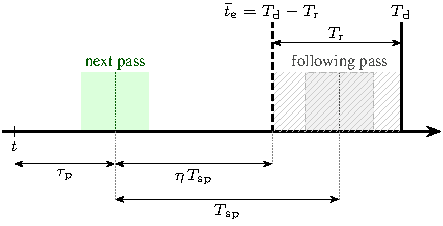
\includegraphics{figures/fig_timeline.pdf}
\caption{Opportunity structure of Problem~1. Passes of the port recur with the spin period $\Ts$; an entry must begin by $\te=\Td-\Tr$. The opportunity margin $\eta$ in \eqref{eq:eta} counts the spin periods left after the next pass; in the case shown, $\eta<1$ and the next pass is the last one.}
\label{fig:timeline}
\end{figure}

Five features follow. 1)~The port sweeps periodically, so the time at which an entry is possible is decided by the rotation of the target. 2)~Whether a pass is usable depends on how closely the line of sight approaches the sweep of the port, and when it occurs depends on the phase of the port. 3)~An entry plan can fail during execution, and abandoning the pass costs about one spin period. 4)~Whether an intent can be converted into an entry is resolved by the execution layer on a time scale of seconds and is not visible in the outcome until much later. 5)~When $\eta<1$, neighboring decisions can lead to capture and timeout, respectively. Features 1--3 raise the question of how to steer the chaser, with a low-dimensional decision, so that passes become usable and correctly timed; Section~\ref{sec:framework} answers it with rotation-synchronized window guidance. Features 4 and 5 raise the question of how a learned decision layer, whose decisions take effect only through the rules of a constrained executor, can account for opportunities that only the executor resolves; Section~\ref{sec:ecc} answers it with execution-feedback closed-loop coordination.

\section{HIERARCHICAL FRAMEWORK AND ROTATION-SYNCHRONIZED WINDOW GUIDANCE}\label{sec:framework}

This section addresses the first question of Section~\ref{sec:mission}. It introduces the hierarchical structure and the interface through which the execution layer serves the decision layer, develops the rotation-synchronized window guidance (RWG) that turns a two-dimensional intent into motion synchronized with the rotating port, and describes the entry logic and the constrained controllers that complete the execution layer. The coupling between the two layers is the subject of Section~\ref{sec:ecc}.

\subsection{Hierarchical Structure and Execution-Layer Interface}\label{sec:integration}

Constrained optimization enforces the constraints of Table~\ref{tab:constraints} explicitly, but in the near field its horizon covers seconds, whereas the value of a decision in Problem~1 depends on whether a pass tens of seconds ahead is used or missed \cite{reiter2026arc,ren2026taes}. A learned policy can represent such long-horizon trade-offs between time, propellant, and opportunity, but learning thrust commands end to end, as in \cite{yang2025taes}, requires extensive interaction and offers limited means to enforce hard constraints \cite{reiter2026arc}. The two roles are therefore assigned to two layers. Once per stage of nominal duration $h$, a learned decision layer issues a stage intent $\ba=[a_{\mathrm{p}},a_{\mathrm{z}}]^{\T}\in\Aset=[-1,1]^{2}$, whose components set the closing pace and the timing of the encounter with the rotating port. An execution layer with fixed parameters converts the intent into constrained motion, decides and plans the entry toward the port, and executes the near-field approach. In the taxonomy of \cite{reiter2026arc}, the decision layer parameterizes an optimization-based executor that is part of the environment during learning. Three design choices shape the structure.

\textit{1) Event-driven macro steps:} A decision is requested at the end of a stage, or earlier when the tracking deviation exceeds $\bar d_{\mathrm{h}}$ and the execution layer switches to hold. Once an entry transfer or the terminal descent has begun, the execution layer continues without further decisions until termination or until the entry is lost. An entry is thus never interrupted by the policy, and the interval between two decisions, called a macro step, has a well-defined outcome: the reward accumulated over it, the successor state, and a termination flag.

\textit{2) Execution modes:} The execution layer operates in the four modes of Table~\ref{tab:modes}, and decisions are taken only in the stage-flight mode $\modeS$ and the hold mode $\modeH$. Translation beyond the range $\rho_{\mathrm{f}}$ is tracked by a feedback law, and the near-field model predictive controller (MPC) acts within $\rho_{\mathrm{f}}$ and throughout the entry transfer $\modeE$ and the terminal descent $\modeD$, where the port-relative constraints become active. A lost entry or an exit from the descent region reverts to $\modeH$.

\textit{3) Multirate operation:} Control and constraint evaluation run every $\Delta t$, mode logic and entry checks every $\Tm$, decisions every stage $h$, and the mode prediction of Section~\ref{sec:screening} covers $\Tp=3h$. The stage is short compared with a pass, so that several decisions precede each pass and the constant-rate prediction \eqref{eq:pred} remains accurate over a stage, and long enough for the attainable velocity change, which grows with $h^{2}$, to reshape the encounter; three stages cover one pass.

\begin{table}
\caption{Execution Modes}
\label{tab:modes}
\tablefont
\begin{tabular*}{\columnwidth}{@{\extracolsep{\fill}}>{\raggedright\arraybackslash}p{4.0pc}>{\raggedright\arraybackslash}p{7.0pc}>{\raggedright\arraybackslash}p{7.0pc}@{}}
\hline
Mode & Entered when & Translation reference\\
\hline
Stage flight $\modeS$ & Stage plan of the new intent is feasible & Stage plan\\
Hold $\modeH$ & Stage plan infeasible, deviation $>\bar d_{\mathrm{h}}$, entry lost, or descent region left & Inertial position at hold onset\\
Entry transfer $\modeE$ & Entry condition \eqref{eq:entry} holds & Entry plan\\
Terminal descent $\modeD$ & $\brhoT\in\Km$, $\rho<\rhos$, or $\brhoT\in\Kset$ with $\rho<\rho_{\mathrm{D}}$ & Lead point on the port axis\\
\hline
\end{tabular*}
\end{table}

The decision layer interacts with the execution layer only through the following interface.

\begin{definition}[Execution-layer interface]\label{def:interface}
Let the decision state $x\in\Xset$ comprise the joint state $X$, the time $t$, the propellant used $\Delta v$, the mission parameters, and the internal state of the execution layer (mode, hold reference, record of the previous stage, and solver warm starts). At a decision state, the execution layer provides:
\begin{enumerate}
\item the macro-step kernel $\PE(x',r\,|\,x,\ba)$ induced by executing an intent $\ba$ from $x$ until the next decision, where $r$ is the reward of the macro step (Section~\ref{sec:mdp});
\item a mode prediction $\Mpred(x,\bb)$ stating whether, when, and at what propellant cost holding an intent $\bb$ would make the execution layer leave stage flight for an entry transfer or the terminal descent within $\Tp$;
\item an execution-feedback vector $\bz(x)$ of opportunity judgments and execution status.
\end{enumerate}
\end{definition}

Because entry transfers and descents run until termination or until the entry is lost, which voids the entry plan, no unfinished entry plan exists at a decision instant, and $x$ determines the evolution of the closed loop over a macro step. Item~1 is what any learning method interacts with; items~2 and~3 are formed from the rules and models of the execution layer itself and are used in Section~\ref{sec:ecc}. The interface does not refer to a particular execution layer; RWG, developed next, is the instance used in this article. Fig.~\ref{fig:framework} shows the resulting architecture.

\begin{figure*}[t]
\centering
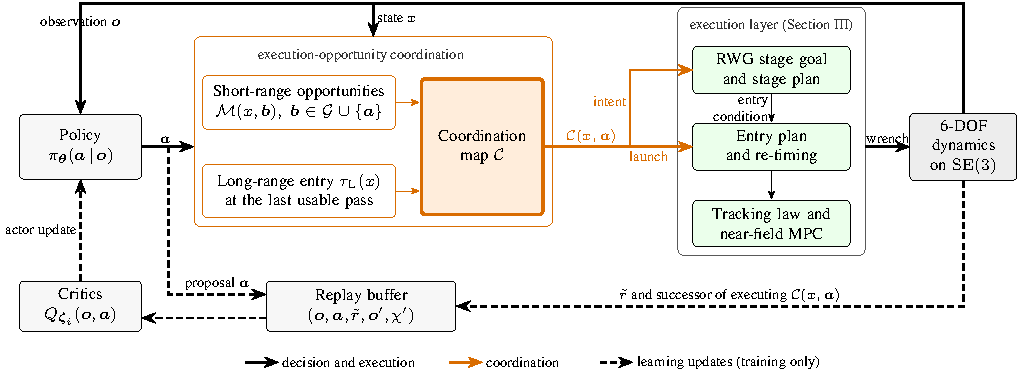
\includegraphics{figures/fig_framework.pdf}
\caption{Execution-aware hierarchical framework. The execution layer exposes the interface of Definition~\ref{def:interface}: the transition of an executed intent, the mode prediction $\Mpred$, and the execution feedback $\bz$. The action-level channel (orange) corrects the proposal $\ba$ into the executed intent $\atil$ in training and execution alike; the state-level channel (blue) feeds $\bz$ to the critics. Dashed paths exist only in training.}
\label{fig:framework}
\end{figure*}

\begin{figure*}[t]
\centering
\begin{minipage}[b]{0.31\textwidth}\centering
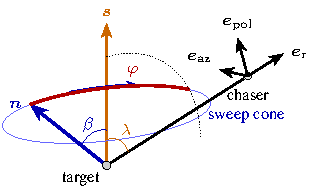
\includegraphics{figures/fig_rwg_a.pdf}\\[2pt]{\footnotesize (a)}
\end{minipage}\hfill
\begin{minipage}[b]{0.35\textwidth}\centering
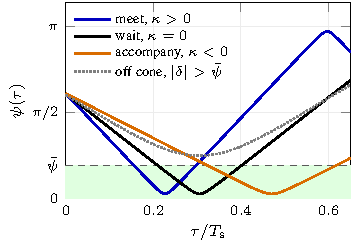
\includegraphics{figures/fig_rwg_b.pdf}\\[2pt]{\footnotesize (b)}
\end{minipage}\hfill
\begin{minipage}[b]{0.33\textwidth}\centering
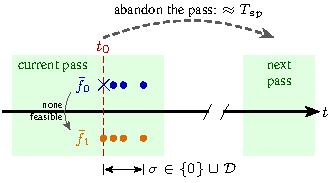
\includegraphics{figures/fig_rwg_c.pdf}\\[2pt]{\footnotesize (c)}
\end{minipage}
\caption{Rotation-synchronized window guidance. (a) Sweep-cone geometry: the port direction $\bn$ rotates about $\bs$ on a cone of half-angle $\beta$; $\lambda$ is the polar angle of the line of sight and $\varphi$ the remaining phase to the pass. (b) Analytic port--line-of-sight angle \eqref{eq:theta} at fixed range under the constant phase rates of Proposition~\ref{prop:rwg}(iii), for $\beta=85^{\circ}$, $\lambda=90^{\circ}$, and $\kappa\in\{0.35,0,-0.35\}$, and for an off-cone line of sight with $|\dlat|>\psig$; the shaded band is the entry gate. (c) Entry re-timing: when the plan arriving at $t_{0}$ is infeasible ($\times$), shifted arrivals with the bounds $\bar f_{0}$ and $\bar f_{1}$ are tried before the pass is abandoned.}
\label{fig:rwg}
\end{figure*}

\subsection{Sweep-Cone Geometry and Rotation-Synchronized Intent}\label{sec:geometry}

RWG addresses Features 1 and 2 of Section~\ref{sec:mission}. Under the prediction \eqref{eq:pred}, the port direction $\bn$ rotates uniformly about $\bs$ and sweeps a cone of half-angle $\beta=\angle(\bn,\bs)$, referred to as the sweep cone. At the relative position $\brho$, a local orthonormal basis is formed by the line-of-sight direction $\er=\brho/\rho$, the unit projection $\epol$ of $\bs$ onto the plane normal to $\er$, and $\eaz=\er\times\epol$, which points toward the oncoming port (Fig.~\ref{fig:rwg}(a)). The geometry is described by the line-of-sight polar angle $\lambda=\angle(\er,\bs)$, the latitude offset $\dlat=\lambda-\beta$, and the phase $\varphi\in[0,2\pi)$ that the port still has to sweep about $\bs$ before it reaches the meridian plane of the line of sight. For the line of sight held fixed, the angle $\psi(\tau)$ between the port direction and $\er$ after a time $\tau$ follows from the spherical law of cosines,
\begin{equation}\label{eq:theta}
\cos\psi(\tau)=\cos\lambda\cos\beta+\sin\lambda\sin\beta\cos(\varphi-\Omega\tau),
\end{equation}
with the phase difference wrapped to $[-\pi,\pi]$. An entry is considered only while $\psi$ is below an entry gate $\psig$.

\begin{lemma}[Passing window]\label{lem:window}
Let $\sin\lambda\sin\beta>0$. If $|\dlat|>\psig$, then $\psi(\tau)>\psig$ for all $\tau$. If $|\dlat|\le\psig$, then $\psi(\tau)\le\psig$ if and only if $|\varphi-\Omega\tau|\le\phw$, where
\begin{equation}\label{eq:halfwidth}
\phw=\arccos\max\Bigl\{-1,\ \frac{\cos\psig-\cos\lambda\cos\beta}{\sin\lambda\sin\beta}\Bigr\};
\end{equation}
each pass thus offers a window of duration $2\phw/\Omega$ centered at $\tau=\varphi/\Omega$, where $\psi$ attains its minimum $|\dlat|$.
\end{lemma}

Lemma~\ref{lem:window} exposes the two levers available to the chaser: the latitude offset decides whether a pass is usable and how closely the port aligns with the line of sight, and the phase decides when the pass occurs. For the spin axes considered, $\dlat=0$ nearly maximizes the window duration (Appendix~\ref{app:proofs}). The time-varying line-of-sight region of multistage MPC approaches to tumbling targets \cite{dong2022aa} plays a similar role, with the difference that here the period of the region is comparable to the deadline, so that a pass is a scarce resource that must be scheduled rather than awaited.

RWG maps the intent to the target velocity at the end of a stage,
\begin{equation}\label{eq:vstar}
\bv^{\star}=-v_{\mathrm{cl}}\,\er+v_{\mathrm{lat}}\,\epol+v_{\mathrm{sw}}\,\eaz,
\end{equation}
with the closing speed $v_{\mathrm{cl}}=v_{0}+v_{\mathrm{a}}a_{\mathrm{p}}$ and the along-sweep speed $v_{\mathrm{sw}}=v_{\mathrm{a}}a_{\mathrm{z}}$ set by the policy, and the latitude speed
\begin{equation}\label{eq:vlat}
v_{\mathrm{lat}}=\sat\bigl(k_{\lambda}\rho\,\dlat;\ \bar v_{\mathrm{lat}}\bigr)
\end{equation}
set by a fixed regulation law with gain $k_{\lambda}$ and saturation level $\bar v_{\mathrm{lat}}$. The three components act on the three quantities of Lemma~\ref{lem:window}.

\begin{proposition}[Nominal window regulation]\label{prop:rwg}
Under the prediction \eqref{eq:pred}, let $\sin\lambda>0$ and resolve the relative velocity as $\bv=v_{\mathrm{r}}\er+v_{\mathrm{pol}}\epol+v_{\mathrm{az}}\eaz$.
\begin{enumerate}
\item The range, the latitude offset, and the phase evolve as
\begin{equation}\label{eq:localkin}
\dot\rho=v_{\mathrm{r}},\qquad \dot{\dlat}=-\frac{v_{\mathrm{pol}}}{\rho},\qquad \dot\varphi=-\Omega-\frac{v_{\mathrm{az}}}{\rho\sin\lambda}.
\end{equation}
\item If $v_{\mathrm{pol}}=v_{\mathrm{lat}}$ follows \eqref{eq:vlat} and $\rho\le\bar\rho_{\mathrm{r}}$, then $|\dlat|$ decreases monotonically, enters the set $|\dlat|\le\bar v_{\mathrm{lat}}/(k_{\lambda}\bar\rho_{\mathrm{r}})$ in finite time, and decays exponentially with rate $k_{\lambda}$ thereafter.
\item If $\rho$ and $\lambda$ are constant and $v_{\mathrm{az}}=v_{\mathrm{sw}}$ is constant with $\kappa=v_{\mathrm{sw}}/(\Omega\rho\sin\lambda)>-1$, then the phase decreases at the rate $\Omega(1+\kappa)$, and the next pass occurs after $\varphi/(\Omega(1+\kappa))$ and lasts $2\phw/(\Omega(1+\kappa))$.
\end{enumerate}
\end{proposition}

The proofs are given in Appendix~\ref{app:proofs}. Proposition~\ref{prop:rwg} assigns one role to each component: $v_{\mathrm{cl}}$ sets the range, $v_{\mathrm{lat}}$ brings the line of sight onto the sweep cone and thereby opens the window of Lemma~\ref{lem:window}, and $v_{\mathrm{sw}}$ places the window in time. Meeting the oncoming port ($\kappa>0$) advances and shortens the pass, accompanying it ($\kappa<0$) delays and lengthens it, and waiting ($\kappa=0$) leaves the natural sweep (Fig.~\ref{fig:rwg}(b)). These are values of one continuous action rather than predefined maneuvers; which of them is preferable depends on the remaining time, the mission, and the propellant, which is the state-dependent decision delegated to learning.

The stage goal is formed from the current state $(\brho,\bv)$ and $\bv^{\star}$ as
\begin{equation}\label{eq:goal}
\begin{aligned}
\bv_{\mathrm{g}}&=\mathcal{P}\bigl(\bv+\sat(\bv^{\star}-\bv;\ \bar v_{\mathrm{st}})\bigr),\\
\brho_{\mathrm{g}}&=\brho+\tfrac{h}{2}(\bv+\bv_{\mathrm{g}}),
\end{aligned}
\end{equation}
where $\bar v_{\mathrm{st}}$ is the velocity change attainable within one stage with a fraction of the planning thrust and $\mathcal{P}$ reduces only the inward radial component of its argument, so that the stage ends at a range of at least $\rho_{\min}>\rhos+\ell_{\mathrm{m}}$ with a radial braking margin of at least $m_{\mathrm{b},\min}$. The operation sphere is thereby entered only through an entry transfer or the terminal descent. The pair $(\brho_{\mathrm{g}},\bv_{\mathrm{g}})$ is the soft terminal target of the stage plan.


\subsection{Dynamic Entry and Entry Re-Timing}\label{sec:entry}

Feature 3 concerns the conversion of a pass into an entry. Both the stage plan and the entry plan are instances of the following subproblem on the double integrator \eqref{eq:di}.

\noindent\textit{Problem~2 (Planning subproblem):} Given the state $(\brho_{0},\bv_{0})$ at time $t$, a horizon $T$ divided into $N$ intervals of length $\Delta t_{\mathrm{pl}}=T/N$, and a thrust bound $\bar f_{\mathrm{pl}}$,
\begin{equation}\label{eq:plan}
\begin{aligned}
\min_{\bff_{0},\dots,\bff_{N-1}}\ \ & L_{\mathrm{f}}(\brho_{N},\bv_{N})+w_{\mathrm{v}}\sum_{n=0}^{N-1}\frac{\norm{\bff_{n}}\Delta t_{\mathrm{pl}}}{\mC}\\
\text{s.t.}\ \ & \eqref{eq:di}\text{ with }\bff\equiv\bff_{n}\text{ on interval }n,\\
& \norm{\bff_{n}}\le\bar f_{\mathrm{pl}},\qquad \rhom\le\rho\le\bar\rho_{\mathrm{pl}},\\
& -\dot\rho\le\vb(\rho-\rhos),\qquad (\brho_{N},\bv_{N})\in\mathcal{X}_{\mathrm{f}},
\end{aligned}
\end{equation}
where the path constraints are imposed at the nodes and at interior points of every interval. The stage plan uses $T=h$, the soft terminal cost $L_{\mathrm{f}}=w_{\rho}\norm{\brho_{N}-\brho_{\mathrm{g}}}^{2}+w_{\mathrm{g}}\norm{\bv_{N}-\bv_{\mathrm{g}}}^{2}$, and no terminal set. The entry plan uses an arrival time $T=\tau$, $L_{\mathrm{f}}=0$, $w_{\mathrm{v}}=1$, and the terminal set that places the chaser at the mouth point $\brhom(t+\tau)=\rhom\hat{\bR}_{\mathrm{T}}(t+\tau)\bnp$ on the port axis outside the operation sphere, moving with it and closing at $v_{\mathrm{in}}$ along the port axis. The keep-out sphere of radius $\rhom$ is nonconvex; following \cite{lian2026asr}, it is linearized at the previous iterate and the problem is solved as a sequence of second-order cone programs. The planning bound $\bar f_{\mathrm{pl}}<\fmax$ leaves a margin for tracking.

While the execution layer is in $\modeS$ or $\modeH$, the entry condition is checked every $\Tm$ once $\rho\le\rho_{\mathrm{E}}$ and the radial braking margin $m_{\mathrm{b}}=\vb(\rho-\rhos)+\dot\rho$ is at least $m_{\mathrm{b},\min}$. The arrival time is the earliest
\begin{equation}\label{eq:entry}
\begin{aligned}
\tau_{\mathrm{e}}=\min\bigl\{\tau\in\Tset:\ &\hat\psi(\tau)\le\psig,\ \ t+\tau\le\te,\\
&\text{Problem~2 is feasible}\bigr\},
\end{aligned}
\end{equation}
where $\Tset$ is a finite set of candidate arrival times, $\hat\psi$ is the angle \eqref{eq:theta} under the prediction \eqref{eq:pred}, and the entry plan uses the bound $\bar f_{0}$. If \eqref{eq:entry} has a solution, the entry transfer starts toward $\brhom(t+\tau_{\mathrm{e}})$. The thresholds $\rho_{\mathrm{E}}$, $\psig$, and $m_{\mathrm{b},\min}$ limit the number of planner calls; safety is defined by Table~\ref{tab:constraints} alone. The latest admissible entry time $\te=\Td-\Tr$ reserves $\Tr$ for the descent.

During the transfer, the entry plan is retained while the tracking deviation stays below $\bar d_{\mathrm{e}}$; otherwise it is re-solved toward the original arrival instant $t_{0}$. If this fails, entry re-timing tries the arrival instants and bounds
\begin{equation}\label{eq:retime}
\begin{aligned}
&(t_{0}+\sigma,\ \bar f_{0}), && \sigma\in\Sigma_{0},\\
&(t_{0}+\sigma,\ \bar f_{1}), && \sigma\in\Sigma_{1}=\{0\}\cup\Sigma_{0},
\end{aligned}
\end{equation}
in this order, subject to $t_{0}+\sigma\le\te$, with shifts $\sigma>0$ in $\Sigma_{0}$ much smaller than $\Ts$ and $\bar f_{0}<\bar f_{1}\le\fmax$. The first feasible candidate is adopted; if none is feasible, the entry is lost and the mode reverts to $\modeH$. Re-timing thus replaces the alternative of abandoning the pass, which costs about one spin period, by a re-plan around the original arrival instant (Fig.~\ref{fig:rwg}(c)).

\begin{remark}\label{rem:retime}
If a feasible entry plan exists with the arrival instant fixed at $t_{0}$, re-timing returns that plan, because its first evaluation is the same convex problem with the same data. For a fixed arrival instant and linearization point, the subproblems with $\bar f_{0}$ and $\bar f_{1}$ differ only in the thrust bound, so the feasible set under $\bar f_{1}$ contains that under $\bar f_{0}$. Re-timing therefore never removes an executable entry. This is a property of the candidate set; it does not imply that the capture rate increases or that a re-timed arrival stays within the same pass.
\end{remark}

\subsection{Constrained Execution Layer}\label{sec:executor}

Beyond $\rho_{\mathrm{f}}$, translation tracks the stage plan in inertial axes by a feedforward and proportional--derivative law, and a pointing controller keeps the boresight on the port. In the terminal descent, the reference is a lead point on the port axis in $\FT$ that advances toward $\bpcap$ at the smaller of the braking-envelope speed and the speed $\fmax/(4\Omega\mC)$ admitted by the Coriolis acceleration.

The near-field MPC computes the full control wrench. Its state is the exponential coordinate of the relative pose and twist $(\bg_{\mathrm{r}},\bxi_{\mathrm{r}})$ in $\FT$, and its prediction model is the relative dynamics linearized at the current state. It minimizes a quadratic cost on the scaled tracking errors and inputs over a horizon of $N_{\mathrm{mpc}}$ control periods, where the translational reference is the plan of the current mode and the attitude reference is the line of sight to the port, switching to the docking attitude in the descent. The constraints comprise the input bounds and the constraints of Table~\ref{tab:constraints} linearized along the predicted trajectory, with the approach cone approximated by a polyhedron and softened by a slack variable. The MPC thus supplies the near-field execution capability, whereas decisions over the horizon of a pass are left to the decision layer.

\section{EXECUTION-FEEDBACK CLOSED-LOOP COORDINATION}\label{sec:ecc}

This section addresses the second question of Section~\ref{sec:mission}. The hierarchy of Section~\ref{sec:framework} separates long-horizon decisions from constrained execution, but it also separates what the two layers know, and a decision layer trained only on realized transitions faces three mismatches with its executor. 1)~\textit{Information:} the execution layer can tell whether an intent will be converted into an entry, whereas the policy must infer this from sparse terminal outcomes; the state-level channel of Section~\ref{sec:feedback} passes this knowledge to the critics. 2)~\textit{Time scale:} decisions are taken once per stage, while passes recur once per spin period; the mode prediction of the execution layer spans $\Tp$, which covers a pass, and the action-level channel of Section~\ref{sec:screening} uses it at every decision. 3)~\textit{Consequence:} when $\eta<1$, neighboring intents can lead to capture and timeout, respectively, so that the value exhibits cliffs located by executor rules; the action-level channel corrects a proposal that would miss the last pass. Because the correction changes the transitions that the policy experiences, learning must take place under the same correction, which is the subject of Section~\ref{sec:consistent}. Learning itself remains off-policy temporal-difference learning on real transitions; the execution layer generates no value labels.

\begin{figure*}[t]
\centering
\begin{minipage}[b]{0.27\textwidth}\centering
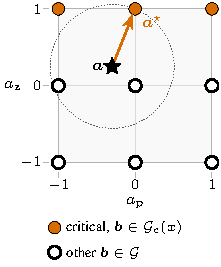
\includegraphics{figures/fig_screen_a.pdf}\\[2pt]{\footnotesize (a)}
\end{minipage}\hfill
\begin{minipage}[b]{0.35\textwidth}\centering
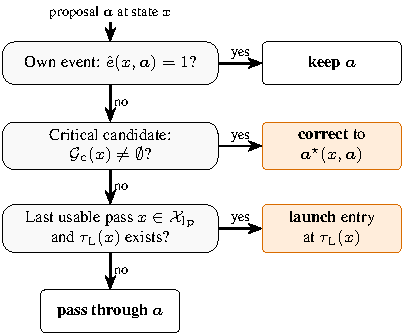
\includegraphics{figures/fig_screen_b.pdf}\\[2pt]{\footnotesize (b)}
\end{minipage}\hfill
\begin{minipage}[b]{0.36\textwidth}\centering
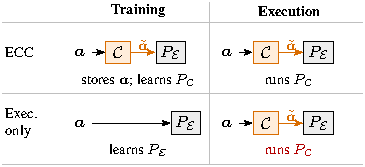
\includegraphics{figures/fig_screen_c.pdf}\\[2pt]{\footnotesize (c)}
\end{minipage}
\caption{Execution-opportunity screening. (a) Correction on the action box: the proposal $\ba$ triggers no mode event and is replaced by the nearest admissible candidate $\atil$; the dotted circle is the distance level set through $\atil$. (b) Critical-window condition of \eqref{eq:admissible}: the event predicted at $t+\tauhat$ is critical because the next pass, one spin period later, falls after $\te$. (c) Kernels learned and executed: with screening in training and execution, the policy is learned and executed under $\PC$; with screening at execution only, it is learned under $\PE$ but executed under $\PC$.}
\label{fig:screen}
\end{figure*}

\subsection{Macro-Step Decision Process}\label{sec:mdp}

Decisions are taken at the instants $t_{k}$ at which a macro step begins in mode $\modeS$ or $\modeH$, with the decision state $x_{k}$ of Definition~\ref{def:interface}. The policy reads the observation
\begin{equation}\label{eq:obs}
\begin{aligned}
\bo=\bigl[&\rho,\ (\bR_{\mathrm{s}}^{\T}\bv)^{\T},\ \psi,\ \dlat,\ \sin\varphi,\ \cos\varphi,\ \Omega,\\
&\Td-t,\ \iota,\ \Delta v,\ \Bmax-\Delta v,\ m_{\mathrm{b}},\ \beta,\ (\bR_{\mathrm{s}}^{\T}\bn)^{\T}\bigr]^{\T},
\end{aligned}
\end{equation}
where $\bR_{\mathrm{s}}=[\er,\epol,\eaz]$ resolves the relative velocity and the port direction in the basis of Section~\ref{sec:geometry}, $\psi=\psi(0)$ is the current port--line-of-sight angle, $\iota\in\{0,1\}$ is a mission indicator that identifies the cost weights, and $m_{\mathrm{b}}$ is the radial braking margin of Section~\ref{sec:entry}. The observation thus expresses the sweep-cone geometry directly, together with the remaining time and propellant; each entry is normalized by a fixed physical scale. The relative attitude is regulated by the execution layer and is not observed by the policy.

The intent $\ba_{k}\in\Aset$ is proposed by the policy and executed, after the correction of Section~\ref{sec:screening}, until the macro step ends. The reward of the macro step is
\begin{equation}\label{eq:reward}
r_{k}=\sum_{j\in\mathcal{J}_{k}}\bigl(-c_{\mathrm{t}}\Delta t-c_{\mathrm{f}}\Delta v_{j}\bigr)+r_{\mathrm{term}},
\end{equation}
where $\mathcal{J}_{k}$ collects the control periods of the macro step, $\Delta v_{j}$ is the velocity increment of period $j$, and $r_{\mathrm{term}}$ is $+100$ at capture, $-100$ at timeout ($t\ge\Td$), $-100$ at fuel exhaustion ($\Delta v\ge\Bmax$), $-150$ at an unsafe state ($X\notin\Sset$), and $0$ otherwise. Each of the four events terminates the process, which is indicated by $\chi_{k+1}=1$. For a captured task, the return $G=\sum_{k}r_{k}$ equals $100$ minus the cost of Problem~1, so that maximizing $\E[G]$ is the penalty form of \eqref{eq:problem}. A constant discount $\gamma$ is applied per decision. Training uses the potential-based shaped reward
\begin{equation}\label{eq:shaping}
\begin{aligned}
\rtil_{k}&=r_{k}+\gamma\Phi(x_{k+1})-\Phi(x_{k}),\\
\Phi(x)&=-\min\bigl\{\bar\ell_{\Phi},\ \norm{\brho-\brhom(t+\tau_{\Phi})}\bigr\},
\end{aligned}
\end{equation}
with $\Phi=0$ at termination, which attracts the chaser toward the mouth point predicted $\tau_{\Phi}$ ahead and leaves the optimal policies unchanged \cite{ng1999shaping}. All evaluations report the return $G$ of the unshaped reward \eqref{eq:reward}.

\subsection{State-Level Channel: Execution Feedback}\label{sec:feedback}

The execution feedback of Definition~\ref{def:interface} consists of three opportunity judgments and three execution-status quantities,
\begin{equation}\label{eq:zE}
\bz=\bigl[\taup,\ \min_{\tau\in\Tset}\hat\psi(\tau),\ \Td-t-\taup-T_{\mathrm{o}},\ d_{\rho},\ d_{v},\ i_{\modeH}\bigr]^{\T}.
\end{equation}
The first item is the time $\taup=\varphi/\Omega$ to the next pass, the second is the closest port alignment over the candidate arrival times of \eqref{eq:entry}, and the third is the deadline margin left after the pass once a fixed time $T_{\mathrm{o}}$ for the final phase is deducted; it differs from $\eta\Ts$ in \eqref{eq:eta} only by the constant $T_{\mathrm{o}}-\Tr$. The remaining items are the position and velocity deviations $d_{\rho}$ and $d_{v}$ of the previous stage from its plan and the indicator $i_{\modeH}\in\{0,1\}$ of the hold mode. The actor and the two critics are
\begin{equation}\label{eq:asym}
\pi_{\vect{\theta}}(\ba\,|\,\bo),\qquad Q_{\vect{\zeta}_{i}}(\bo,\bz,\ba),\quad i=1,2.
\end{equation}
For the same observation, $\bz$ distinguishes whether an opportunity actually exists and whether the previous intent was executed as planned, so that the critics can represent values closer to the realized consequences of execution. The feedback is used only by the critics during training; at execution, the policy acts on $\bo$ alone.

\subsection{Action-Level Channel: Execution-Opportunity Screening}\label{sec:screening}

The action-level channel rests on a question that the execution layer answers from its own rules: if an intent were held from now on, would the execution layer leave stage flight, and if so, when and at what propellant cost?

\begin{definition}[Mode prediction]\label{def:pred}
The mode prediction is the map $\Mpred:\Xset\times\Aset\to\{0,1\}\times[0,\Tp]\times\R_{\ge0}$, $(x,\bb)\mapsto(\ehat,\tauhat,\dvhat)$, where $\ehat=1$ if and only if, under the prediction \eqref{eq:pred} and with the intent $\bb$ held, the rules of Section~\ref{sec:framework} produce the terminal descent or a feasible entry within $\Tp$, $\tauhat$ is the time of this event or the time at which the prediction stops, and $\dvhat$ is the planned velocity increment up to the event, including the entry plan.
\end{definition}

The prediction rolls out the stage goals \eqref{eq:goal} and the stage plans of Problem~2 for up to $\Tp/h$ stages, treating a rejected stage as a hold, and applies the descent condition of Table~\ref{tab:modes} and the entry condition \eqref{eq:entry} every $\Tm$ along the planned path. It stops at the first event, at $\Tp$, at the deadline, or when the planned propellant exhausts the budget. It uses no data from past tasks, evaluates no rewards or values, and runs on separate planner instances, so that the executed trajectory is the same whether or not a prediction is made. A predicted event is a mode switch in the model of the execution layer, not a capture.

Let $\Gset\subset\Aset$ be a finite set of candidate intents; this article uses the uniform grid $\Gset=\{-1,0,1\}^{2}$, which covers the action box with its center, edges, and vertices. The admissible candidate set is
\begin{equation}\label{eq:admissible}
\begin{aligned}
\Ga(x)=\bigl\{\bb\in\Gset:\ & \ehat(x,\bb)=1,\ \ t+\tauhat(x,\bb)+\Ts>\te,\\
& \Delta v+\dvhat(x,\bb)\le\Bmax\bigr\}.
\end{aligned}
\end{equation}
The three conditions require that the candidate trigger an entry or a descent, that the event belong to a critical window, and that the candidate be affordable. The second condition is the predicted counterpart of $\eta<1$ in \eqref{eq:eta}: with the predicted event in place of the pass center, it states that missing the event leaves no further pass before $\te$ (Fig.~\ref{fig:screen}(b)). The correction map is
\begin{equation}\label{eq:correction}
\Cmap(x,\ba)=
\begin{cases}
\ba, & \text{if }\ehat(x,\ba)=1\text{ or }\Ga(x)=\emptyset,\\
\ba^{\star}(x,\ba), & \text{otherwise},
\end{cases}
\end{equation}
with $\ba^{\star}(x,\ba)\in\argmin_{\bb\in\Ga(x)}\norm{\bb-\ba}$,
where ties in the minimization are broken by the smaller $\tauhat(x,\bb)$ and then by a fixed order of $\Gset$. The executed intent is $\atil=\Cmap(x,\ba)$ (Fig.~\ref{fig:screen}(a)); the correction applies to the current macro step only.

\begin{property}\label{prop:correction}
For every $x\in\Xset$ and $\ba\in\Aset$: (i)~$\Cmap(x,\ba)=\ba$ if $\ehat(x,\ba)=1$ or $\Ga(x)=\emptyset$; (ii)~otherwise $\Cmap(x,\ba)\in\Ga(x)$ and $\norm{\Cmap(x,\ba)-\ba}=\min_{\bb\in\Ga(x)}\norm{\bb-\ba}$; (iii)~$\Cmap$ is single valued and idempotent, $\Cmap(x,\Cmap(x,\ba))=\Cmap(x,\ba)$.
\end{property}

Items (i) and (ii) restate \eqref{eq:correction}; the minimizer exists because $\Ga(x)$ is finite. The tie-breaking rule and the deterministic prediction make $\Cmap$ single valued, and a corrected intent lies in $\Ga(x)$, so it triggers an event and is left unchanged by a second application. Screening therefore acts only when the proposal would miss a critical window that a candidate can use, and then changes the intent as little as the candidate set allows. Each decision requires $|\Gset|+1$ mode predictions, each with at most $\Tp/h$ stage plans and $|\Tset|\Tp/\Tm$ entry plans. Screening is a test on the model of the execution layer; it guarantees neither safety nor capture.


\subsection{Training--Execution Consistent Learning}\label{sec:consistent}

Screening modifies the transitions of the closed loop. Applied only at execution, it acts as a postprocessing filter that is invisible during learning, and the policy is optimized for a system other than the one it controls \cite{reiter2026arc}. ECC applies the same map $\Cmap$ in training and execution (Fig.~\ref{fig:screen}(c)). The screened kernel is
\begin{equation}\label{eq:PC}
\PC(x',r\,|\,x,\ba)=\PE\bigl(x',r\,|\,x,\Cmap(x,\ba)\bigr),
\end{equation}
and the replay buffer stores the proposed intent $\ba$, not $\atil$, together with the reward and the successor obtained by executing $\atil$. The critics thus learn what happens when the policy proposes $\ba$.

\begin{proposition}[Screened decision process]\label{prop:screen}
Let transitions be collected by proposing $\ba_{k}\sim\pi(\cdot\,|\,\bo_{k})$, executing $\Cmap(x_{k},\ba_{k})$, and storing $(\bo_{k},\bz_{k},\ba_{k},\rtil_{k},\bo_{k+1},\bz_{k+1},\chi_{k+1})$.
\begin{enumerate}
\item The stored transitions are samples of the decision process $(\Xset,\Aset,\PC,\rtil,\gamma)$, and the temporal-difference target formed from a stored transition is a sample of its Bellman operator
\begin{equation}\label{eq:bellman}
(\mathcal{B}^{\pi}Q)(x,\ba)=\E_{\PC}\Bigl[\rtil+\gamma(1-\chi')\,\E_{\ba'\sim\pi}Q(x',\ba')\Bigr].
\end{equation}
\item If $\Cmap(x,\ba_{1})=\Cmap(x,\ba_{2})$, then $\PC(\cdot\,|\,x,\ba_{1})=\PC(\cdot\,|\,x,\ba_{2})$ and $Q^{\pi}_{\mathcal{C}}(x,\ba_{1})=Q^{\pi}_{\mathcal{C}}(x,\ba_{2})$ for every policy $\pi$.
\item Let $\Pi$ be a class of observation-feedback policies and $V_{\mathcal{C}}(\pi)$ and $V_{\mathcal{E}}(\pi)$ the expected discounted returns of $\pi$ under $\PC$ and $\PE$. The system executed with screening attains $V_{\mathcal{C}}(\pi)$ for every $\pi\in\Pi$; hence any $\pi_{\mathcal{C}}\in\argmax_{\Pi}V_{\mathcal{C}}$ performs on it at least as well as every policy of $\Pi$, including any $\pi_{\mathcal{E}}\in\argmax_{\Pi}V_{\mathcal{E}}$.
\end{enumerate}
\end{proposition}

\textit{Proof:} (i)~By Definition~\ref{def:interface}, $x_{k}$ determines the evolution over a macro step once the executed intent is fixed. The mode prediction runs on separate planner instances and leaves $x_{k}$ unchanged, and $\Cmap$ is a deterministic function of $(x_{k},\ba_{k})$ by Property~\ref{prop:correction}. Hence, conditioned on $(x_{k},\ba_{k})$, the pair $(x_{k+1},r_{k})$ is distributed according to $\PE(\cdot\,|\,x_{k},\Cmap(x_{k},\ba_{k}))=\PC(\cdot\,|\,x_{k},\ba_{k})$, regardless of how $\ba_{k}$ was sampled. The shaped reward is a function of $(x_{k},r_{k},x_{k+1})$ and $\chi_{k+1}$ a function of $x_{k+1}$, so the stored transitions are samples of this decision process, and the target $\rtil_{k}+\gamma(1-\chi_{k+1})\E_{\ba'\sim\pi}Q(x_{k+1},\ba')$ is a sample of \eqref{eq:bellman} at $(x_{k},\ba_{k})$. (ii)~By \eqref{eq:PC}, $\PC(\cdot\,|\,x,\ba)$ depends on $\ba$ only through $\Cmap(x,\ba)$, and so does the fixed point of \eqref{eq:bellman}. (iii)~At execution, a proposal $\ba\sim\pi(\cdot\,|\,\bo)$ is executed as $\Cmap(x,\ba)$, so the executed system follows $\PC$ and its return under $\pi$ is $V_{\mathcal{C}}(\pi)$; the inequality is the definition of a maximizer. Since the shaped and unshaped returns of any policy differ by $-\E[\Phi(x_{0})]$, the maximizers are the same for both rewards. \hfill$\square$

By Proposition~\ref{prop:screen}(ii), proposals mapped to the same candidate have the same value, so the policy need not learn to emit the corrected intent itself; policy and correction act as one decision rule. Proposition~\ref{prop:screen}(iii) states the consequence for the alternatives: a policy trained without screening and executed with it is in general not the best policy for the system it controls, and a policy trained with screening is matched to that system, so that removing screening at execution changes the system it was trained for. It compares optimal values under screening and does not compare a system with screening to one without it.

\begin{remark}\label{rem:related}
Asymmetric actor--critic methods train the critic on privileged simulator states \cite{pinto2018asymmetric}, shielding places a correction layer in the learning loop to enforce safety specifications \cite{alshiekh2018shielding}, postprocessing filters correct actions only at execution \cite{reiter2026arc}, and projection-based schemes learn from the corrected action or a mixture of corrected and original actions \cite{lu2025eaai}. The novelty of ECC lies in their combination for hierarchical RL--MPC. Both channels are supplied by the same execution-layer interface from the short-horizon prediction of the executor itself, rather than from simulator states or a separately synthesized monitor; the correction targets execution opportunities rather than safety, with a criterion derived from the time structure of the task; and the correction is placed so that the learning target is consistent with the executed system (Proposition~\ref{prop:screen}).
\end{remark}

The decision layer is trained with soft actor--critic (SAC) \cite{haarnoja2018sac} in the asymmetric form \eqref{eq:asym}. The policy is a Gaussian squashed by $\tanh$ onto $\Aset$, and the actor and the critics are fully connected networks with separate input layers. With target critics $Q_{\vect{\zeta}_{i}^{-}}$, the critic target and the losses are
\begin{align}
y&=\rtil+\gamma(1-\chi')\Bigl[\min_{i}Q_{\vect{\zeta}_{i}^{-}}(\bo',\bz',\ba')\nonumber\\
&\qquad\qquad-\alpha\log\pi_{\vect{\theta}}(\ba'\,|\,\bo')\Bigr],\label{eq:target}\\
\mathcal{L}(\vect{\zeta}_{i})&=\E\bigl[(Q_{\vect{\zeta}_{i}}(\bo,\bz,\ba)-y)^{2}\bigr],\nonumber\\
\mathcal{L}(\vect{\theta})&=\E\Bigl[\alpha\log\pi_{\vect{\theta}}(\ba_{\theta}\,|\,\bo)-\min_{i}Q_{\vect{\zeta}_{i}}(\bo,\bz,\ba_{\theta})\Bigr],\nonumber
\end{align}
where $\ba'\sim\pi_{\vect{\theta}}(\cdot\,|\,\bo')$, $\ba_{\theta}\sim\pi_{\vect{\theta}}(\cdot\,|\,\bo)$, $\alpha$ is a fixed temperature, and the expectations are taken over the replay buffer. Algorithm~\ref{alg:ecc} summarizes training and execution; at execution, the policy mean is used.

\begin{remark}\label{rem:scope}
Proposition~\ref{prop:screen} concerns the learning target on the decision state $x$; the actor on $\bo$ and the critics on $(\bo,\bz)$ are function approximations of it. No statement is made on the convergence of SAC, on safety, which is judged only on the dynamics \eqref{eq:kin}--\eqref{eq:fg}, or on whether screening improves over its absence; these effects are quantified in Section~\ref{sec:experiments}.
\end{remark}

\begin{algorithm}[t]
\caption{ECC Training and Execution}
\label{alg:ecc}
\small
\begin{algorithmic}[1]
\State Initialize $\pi_{\vect{\theta}}$, $Q_{\vect{\zeta}_{1}},Q_{\vect{\zeta}_{2}}$, targets, and buffer $\mathcal{D}$ \Comment{T}
\For{each decision in mode $\modeS$ or $\modeH$}
  \State Observe $\bo$ (and $\bz$ in training); propose $\ba\sim\pi_{\vect{\theta}}(\cdot\,|\,\bo)$ (mean at execution)
  \State Evaluate $\Mpred(x,\bb)$ for $\bb\in\Gset\cup\{\ba\}$; form $\Ga(x)$ by \eqref{eq:admissible}
  \State Set $\atil\gets\Cmap(x,\ba)$ by \eqref{eq:correction}
  \State Execute $\atil$ with RWG and MPC until the macro step ends
  \State Store $(\bo,\bz,\ba,\rtil,\bo',\bz',\chi')$ in $\mathcal{D}$ \Comment{T}
  \State Update the critics and the actor by \eqref{eq:target} \Comment{T}
\EndFor
\end{algorithmic}
\textit{Note:} Steps marked T are performed only in training; all other steps are shared by training and execution.
\end{algorithm}

\section{NUMERICAL SIMULATIONS}\label{sec:experiments}

\todo{Section V is written after the formal experiments are delivered. Planned subsections (EXPERIMENTS.md, Sections 1--3 and 5--7): A) setup, compared methods, and training (Table of settings, F1); B) representative case (F2--F3); C) main results on urgent and economy missions (F4, T2); D) attribution and ablations (F6); E) mechanism and operating boundary (F5, F7, computational cost).}

\section{CONCLUSION}\label{sec:conclusion}

This article studied the pre-capture approach to a target that tumbles fast enough for its docking port to face the chaser only once per spin period, a period comparable to the deadline of the task. The proposed framework assigns the long-horizon decisions to a learned policy and the constrained motion to an execution layer of planners and MPC, and connects the two layers in both directions. RWG expresses the decisions in terms of the sweep-cone geometry: the latitude of the line of sight is regulated onto the cone swept by the port, the policy sets the closing pace and the timing of the encounter, and entries are planned toward the predicted port motion and re-timed within the same pass. ECC returns to every decision the entry opportunities that the execution layer can realize, keeps, corrects, or replaces the proposed intent by one rule, and trains the policy on the coordinated closed loop with the proposal stored, so that the critics learn the consequences of proposals under coordination with standard SAC losses.

In six-degree-of-freedom simulations of time-limited pre-capture, ECC captured $85.4\%$ of the test tasks against $73.8\%$ for learning-guided MPC on the same execution chain, $63.9\%$ with TD3, and $44.3\%$ for MPC alone. The gain consists of tasks captured in time, at the same completion time and propellant per capture, and it is concentrated in the tighter deadlines, where few passes remain. RWG raised the captures of a fixed intent from $64$ to $103$ of $192$ tasks, and entry re-timing added a small positive gain. ECC kept its capture rate under a slower spin and under a stronger nutation outside the training distribution, where the margin over learning-guided MPC grew to $22.4$ and $14.4$ percentage points.

The results are obtained in simulation with the relative state measured without noise, and the execution layer predicts the target attitude at constant angular velocity with an isotropic inertia estimate. Each learning method was trained with three seeds, and the confidence intervals reflect the variation over initial conditions. Of the $192$ test initial conditions, $191$ were captured by at least one method or training run, whereas ECC captured $152$ in all three runs and missed $19$ in all three; the remaining gap lies mainly in the consistency of learning. Future work will combine the coordination with onboard estimation of the target motion under sensing noise and improve the consistency of the learned policies across training runs.

\appendices

\section{PROOFS}\label{app:proofs}

\textit{Proof of Lemma~\ref{lem:window}:} Let $\vect{k}_{1}$ be the unit vector orthogonal to $\bs$ in the meridian plane of the line of sight and $\vect{k}_{2}=\bs\times\vect{k}_{1}$, so that $\er=\cos\lambda\,\bs+\sin\lambda\,\vect{k}_{1}$. Under \eqref{eq:pred}, the port direction after a time $\tau$ is $\hat{\bn}(\tau)=\cos\beta\,\bs+\sin\beta\,(\cos(\Omega\tau-\varphi)\,\vect{k}_{1}+\sin(\Omega\tau-\varphi)\,\vect{k}_{2})$, and $\cos\hat\psi(\tau)=\hat{\bn}(\tau)^{\T}\er$ gives \eqref{eq:theta}. Let $c_{\mathrm{w}}=(\cos\psig-\cos\lambda\cos\beta)/(\sin\lambda\sin\beta)$. Since $\sin\lambda\sin\beta>0$ and the cosine decreases on $[0,\pi]$, $\hat\psi(\tau)\le\psig$ is equivalent to $\cos(\varphi-\Omega\tau)\ge c_{\mathrm{w}}$. Because $\cos\lambda\cos\beta+\sin\lambda\sin\beta=\cos\dlat$ and $|\dlat|,\psig\in[0,\pi]$, $c_{\mathrm{w}}>1$ is equivalent to $|\dlat|>\psig$, in which case no $\tau$ satisfies the inequality. If $c_{\mathrm{w}}\le-1$, it holds for every $\tau$, consistent with $\phw=\pi$. Otherwise, with the phase difference taken modulo $2\pi$ in $[-\pi,\pi]$, it holds if and only if $|\varphi-\Omega\tau|\le\arccos c_{\mathrm{w}}=\phw$, an interval of length $2\phw/\Omega$ centered at $\tau=\varphi/\Omega$, where $\cos\hat\psi=\cos\dlat$, and repeated with the period $\Ts$. \hfill$\square$

\textit{Window duration and latitude offset:} Since $\partial c_{\mathrm{w}}/\partial\lambda=(\cos\beta-\cos\psig\cos\lambda)/(\sin^{2}\lambda\sin\beta)$, for fixed $\beta$ the half-width $\phw$ is largest at $\cos\lambda=\cos\beta/\cos\psig$, which differs from $\lambda=\beta$. With the port axis along the body $x$-axis and the nominal spin-axis offsets of $10$--$20^{\circ}$ (Section~\ref{sec:setup}), $\beta\in[70^{\circ},110^{\circ}]$; over this range and with $\psig=35^{\circ}$, the maximizer lies within $5^{\circ}$ of $\lambda=\beta$, and $\phw$ at $\dlat=0$ is within $0.3^{\circ}$ of its maximum, so that $\dlat=0$ nearly maximizes the window duration for the nominal tumbling.

\textit{Proof of Proposition~\ref{prop:rwg}:} (i)~The relation $\dot\rho=\er^{\T}\bv=v_{\mathrm{r}}$ is immediate, and $\dot{\vect{e}}_{\mathrm{r}}=(\bv-v_{\mathrm{r}}\er)/\rho$. Since $\bs=\cos\lambda\,\er+\sin\lambda\,\epol$, differentiating $\cos\lambda=\bs^{\T}\er$ with $\bs$ fixed gives $-\sin\lambda\,\dot\lambda=\bs^{\T}\dot{\vect{e}}_{\mathrm{r}}=\sin\lambda\,v_{\mathrm{pol}}/\rho$, i.e., $\dot\lambda=-v_{\mathrm{pol}}/\rho$, and $\dot{\dlat}=\dot\lambda$ because $\beta$ is constant under \eqref{eq:pred}. Let $\varphi_{\mathrm{r}}$ be the azimuth of $\er$ about $\bs$, so that $\partial\er/\partial\varphi_{\mathrm{r}}=\bs\times\er$ with $\norm{\bs\times\er}=\sin\lambda$ and $\eaz=-\bs\times\er/\sin\lambda$. Projecting $\dot{\vect{e}}_{\mathrm{r}}$ onto $\bs\times\er$ yields $\sin^{2}\lambda\,\dot\varphi_{\mathrm{r}}=-\sin\lambda\,v_{\mathrm{az}}/\rho$. The phase is the azimuth of the line of sight relative to that of the port, which advances at the rate $\Omega$; this gives the third relation of \eqref{eq:localkin}.

(ii)~With $v_{\mathrm{pol}}=\mathrm{sgn}(\dlat)\min\{k_{\lambda}\rho|\dlat|,\bar v_{\mathrm{lat}}\}$, item~(i) gives $\dd|\dlat|/\dd t=-\min\{k_{\lambda}|\dlat|,\bar v_{\mathrm{lat}}/\rho\}<0$ for $\dlat\neq0$. Let $\bar\dlat=\bar v_{\mathrm{lat}}/(k_{\lambda}\bar\rho)$. Since $\rho\le\bar\rho$, while $|\dlat|>\bar\dlat$, $\dd|\dlat|/\dd t\le-\bar v_{\mathrm{lat}}/\bar\rho$, so $|\dlat|$ reaches $\bar\dlat$ within $(|\dlat(0)|-\bar\dlat)\bar\rho/\bar v_{\mathrm{lat}}$. Once $|\dlat|\le\bar\dlat$, $k_{\lambda}\rho|\dlat|\le\bar v_{\mathrm{lat}}$, the law is unsaturated, and $\dot{\dlat}=-k_{\lambda}\dlat$; since $|\dlat|$ keeps decreasing, the set is not left.

(iii)~With $\rho$, $\lambda$, and $v_{\mathrm{az}}=v_{\mathrm{sw}}$ constant, item~(i) gives $\dot\varphi=-\Omega(1+\kappa)$. Because $\lambda$ and $\beta$ are constant, the predicted port--line-of-sight angle obeys \eqref{eq:theta} with $\Omega\tau$ replaced by $\Omega(1+\kappa)\tau$, and Lemma~\ref{lem:window} applies with the rate $\Omega(1+\kappa)>0$. \hfill$\square$

\section{ECC WITHOUT CRITICAL-WINDOW CORRECTION}\label{app:nocorr}

A variant of ECC that keeps a proposal reaching an event by itself and launches the long-range entry at the last usable pass, but never corrects an intent, was trained from zero with three seeds and evaluated on the same test tasks. It captures $505$ of $576$ tasks ($87.7\%$) against $492$ ($85.4\%$) for ECC, a paired difference of $-2.3$~pp $[-4.2,-0.3]$ for ECC, with the two groups of policies trained separately. Both forms of coordination improve clearly on SAC--MPC without coordination ($425$ captures).

\section{ADDITIONAL PARAMETERS}\label{app:params}

Table~\ref{tab:params2} lists the parameters of the execution layer and of training that complement Table~\ref{tab:params}.

\begin{table}[h]
\caption{Execution-Layer and Training Parameters}
\label{tab:params2}
\tablefont
\setlength{\tabcolsep}{3pt}
\begin{tabular*}{\columnwidth}{@{\extracolsep{\fill}}>{\raggedright\arraybackslash}p{9.5pc}>{\raggedright\arraybackslash}p{9.9pc}@{}}
\hline
Parameter & Value\\
\hline
Target size; rod radius & $1.24\times1.02\times0.74$ m; $0.05$ m\\
$\bpport$; $\bpcap$; $\bnp$ (in $\FT$) & $[-1.5,0,0]^{\T}$ m; $[-3,0,0]^{\T}$ m; $[-1,0,0]^{\T}$\\
Chaser inertia & $\approx\diag(20.3,19.9,23.7)$ kg$\cdot$m$^{2}$\\
Mouth point $\rhom$; inward speed; $v_{\mathrm{mg},\min}$ & $6.3$ m; $0.02$ m/s; $0.02$ m/s\\
Hold deviation; near-field range; descent range & $3$ m; $7.5$ m; $7$ m\\
Entry re-plan deviation; re-timing delays & $1$ m; $\{2,4,8\}$ s\\
Planning intervals $N$: stage; entry & $16$; $30$\\
Stage-plan weights (position, velocity; $w$) & $10$, $200$; $0.1$\\
Range penalty above $20$ m; SCP iterations & $0.01$; $4$\\
Far-field tracking; pointing gains & $\omega_{n}=0.2$ rad/s, critically damped; $0.36$ s$^{-2}$, $1.2$ s$^{-1}$\\
MPC state scales in $\vect{W}$ & $75^{\circ}$, $20$ m, $0.05$ rad/s, $1.1$ m/s\\
$w_{\mathrm{u}}$; $w_{N}$; $w_{\varepsilon}$; $\bar\varepsilon$ & $0.01$; $1000$; $10^{4}$; $2$\\
Cone faces; tightening & $8$; $0.02$\\
Learning rate; batch; buffer & $3\times10^{-4}$; $256$; $10^{5}$\\
Warm-up; updates per transition; target rate & $200$ decisions; $2$; $0.005$\\
\hline
\end{tabular*}
\end{table}


\bibliographystyle{IEEEtaes}
\bibliography{refs}

\end{document}
